\ProblemHeading

\textbf{1.} Determine how many energy levels have each possible value of the total spin $S$ in a system of $N$ particles of spin $1/2$ (F.~Bloch, 1929).

\SolutionHeading A prescribed value of the total-spin projection $M_S=\sum\sigma$ can be formed in
\[
 f(M_S)=\frac{N!}{(N/2+M_S)!(N/2-M_S)!}
\]

\SourcePage{294}{297}
different ways: assign $\sigma=1/2$ to $N/2+M_S$ particles and $\sigma=-1/2$ to all the others. Every energy level of total spin $S$ supplies $2S+1$ states whose projections are $M_S=S,S-1,\ldots,-S$. It follows directly that the number of distinct levels having this value of $S$ is
\[
 n(S)=f(S)-f(S+1)=\frac{N!(2S+1)}{(N/2+S+1)!(N/2-S)!}.
\]
The total number $n=\sum_S n(S)$ of distinct energy levels is
\[
 n=f(0)=\frac{N!}{[(N/2)!]^2}
\]
when $N$ is even, and
\[
 n=f(1/2)=\frac{N!}{[(N+1)/2]![(N-1)/2]!}
\]
when $N$ is odd.

\textbf{2.} Find the total-spin values $S$ that occur for the different symmetry types of the spin functions of a system consisting of two, three, or four particles, each of spin 1.

\SolutionHeading For two particles, the correspondence follows by requiring the multiplier acquired by the spin function upon interchange of the particles to equal $(-1)^{2s-S}$ (see the end of §~62). Thus, for particles of spin $s=1$, the correspondence is
\begin{center}
\begin{tikzpicture}[x=5mm,y=5mm,line width=.35pt]
\node at (-.5,.5) {$a$}; \draw (0,0) rectangle (2,-1); \draw (1,0)--(1,-1); \node at (1,-1.6) {$S=0,2$};
\node at (4-.5,.5) {$b$}; \draw (4,0) rectangle (5,-2); \draw (4,-1)--(5,-1); \node at (4.5,-2.6) {$S=1$}; \node at (8,0) {(1)};
\end{tikzpicture}
\end{center}

The Young diagrams for three particles are obtained by adjoining one cell, in every possible way, to the diagrams in (1). Symbolically, this can be written
\begin{center}
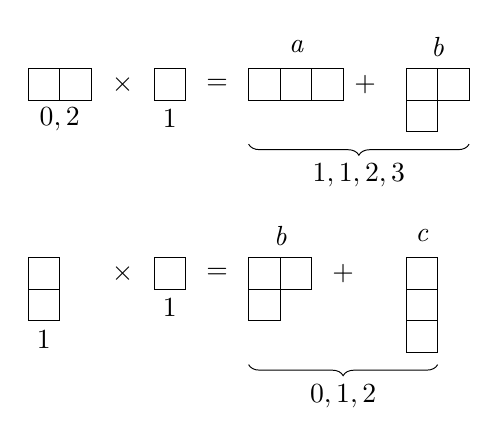
\begin{tikzpicture}[x=4mm,y=4mm,line width=.35pt]
\draw (0,0) rectangle (2,-1);\draw (1,0)--(1,-1);\node at (1,-1.6){$0,2$};\node at (3,-.5){$\times$};\draw (4,0) rectangle (5,-1);\node at (4.5,-1.6){$1$};\node at (6,-.5){$=$};
\node at (8.5,.7){\itshape a};\draw (7,0) rectangle (10,-1);\draw (8,0)--(8,-1);\draw (9,0)--(9,-1);\node at (10.7,-.5){$+$};
\node at (13,.7){\itshape b};\draw (12,0) rectangle (14,-1);\draw (13,0)--(13,-1);\draw (12,-1) rectangle (13,-2);
\draw[decorate,decoration={brace,mirror,amplitude=4pt}] (7,-2.4)--(14,-2.4);\node at (10.5,-3.4){$1,1,2,3$};
\draw (0,-6) rectangle (1,-8);\draw (0,-7)--(1,-7);\node at (.5,-8.6){$1$};\node at (3,-6.5){$\times$};\draw (4,-6) rectangle (5,-7);\node at (4.5,-7.6){$1$};\node at (6,-6.5){$=$};
\node at (8,-5.3){\itshape b};\draw (7,-6) rectangle (9,-7);\draw (8,-6)--(8,-7);\draw (7,-7) rectangle (8,-8);\node at (10,-6.5){$+$};
\node at (12.5,-5.3){\itshape c};\draw (12,-6) rectangle (13,-9);\draw (12,-7)--(13,-7);\draw (12,-8)--(13,-8);
\draw[decorate,decoration={brace,mirror,amplitude=4pt}] (7,-9.4)--(13,-9.4);\node at (10,-10.4){$0,1,2$};
\end{tikzpicture}
\end{center}
The values of $S$ are written below the diagrams. The total spins for the three-particle system (the diagrams on the right) are obtained from the spins of the two-particle and one-particle systems (on the left) by the rule for addition of angular momenta.\footnote{The value 1 occurs twice below the diagrams on the right because it is produced once by adding angular momenta 0 and 1, and once by adding angular momenta 2 and 1.} To distribute

\SourcePage{295}{298}
the resulting values of $S$ among the individual diagrams on the right, observe first that diagram $c$ (a column of three cells) corresponds to $S=0$. Diagram $b$ must therefore receive the remaining values 1 and 2 from the second equality; diagram $a$ then receives the values 1 and 3 left by $b$ in the first equality:
\begin{center}
\begin{tikzpicture}[x=5mm,y=5mm,line width=.35pt]
\node at (-.5,.5){$a$};\draw (0,0) rectangle (3,-1);\draw (1,0)--(1,-1);\draw (2,0)--(2,-1);\node at (1.5,-1.6){$S=1,3$};
\node at (4.5,.5){$b$};\draw (5,0) rectangle (7,-1);\draw (6,0)--(6,-1);\draw (5,-1) rectangle (6,-2);\node at (6,-2.6){$S=1,2$};
\node at (9.5,.5){$c$};\draw (10,0) rectangle (11,-3);\draw (10,-1)--(11,-1);\draw (10,-2)--(11,-2);\node at (10.5,-3.6){$S=0$};
\end{tikzpicture}
\end{center}

The Young diagrams for four particles result from adding one cell to the diagrams in (2), subject to the restriction that no column may contain more than three cells:
\begin{center}
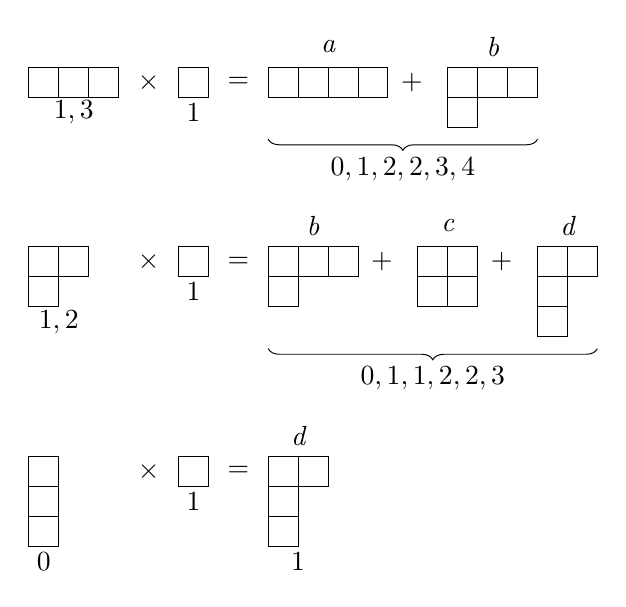
\begin{tikzpicture}[x=3.8mm,y=3.8mm,line width=.35pt]
\draw (0,0) rectangle (3,-1);\draw (1,0)--(1,-1);\draw (2,0)--(2,-1);\node at (1.5,-1.5){$1,3$};\node at (4,-.5){$\times$};\draw (5,0) rectangle (6,-1);\node at (5.5,-1.5){$1$};\node at (7,-.5){$=$};
\node at (10,.7){\itshape a};\draw (8,0) rectangle (12,-1);\foreach \x in {9,10,11}\draw (\x,0)--(\x,-1);\node at (12.8,-.5){$+$};
\node at (15.5,.7){\itshape b};\draw (14,0) rectangle (17,-1);\draw (15,0)--(15,-1);\draw (16,0)--(16,-1);\draw (14,-1) rectangle (15,-2);
\draw[decorate,decoration={brace,mirror,amplitude=4pt}] (8,-2.4)--(17,-2.4);\node at (12.5,-3.4){$0,1,2,2,3,4$};
\draw (0,-6) rectangle (2,-7);\draw (1,-6)--(1,-7);\draw (0,-7) rectangle (1,-8);\node at (1,-8.5){$1,2$};\node at (4,-6.5){$\times$};\draw (5,-6) rectangle (6,-7);\node at (5.5,-7.5){$1$};\node at (7,-6.5){$=$};
\node at (9.5,-5.3){\itshape b};\draw (8,-6) rectangle (11,-7);\draw (9,-6)--(9,-7);\draw (10,-6)--(10,-7);\draw (8,-7) rectangle (9,-8);\node at (11.8,-6.5){$+$};
\node at (14,-5.3){\itshape c};\draw (13,-6) rectangle (15,-8);\draw (14,-6)--(14,-8);\draw (13,-7)--(15,-7);\node at (15.8,-6.5){$+$};
\node at (18,-5.3){\itshape d};\draw (17,-6) rectangle (19,-7);\draw (18,-6)--(18,-7);\draw (17,-7) rectangle (18,-9);\draw (17,-8)--(18,-8);
\draw[decorate,decoration={brace,mirror,amplitude=4pt}] (8,-9.4)--(19,-9.4);\node at (13.5,-10.4){$0,1,1,2,2,3$};
\draw (0,-13) rectangle (1,-16);\draw (0,-14)--(1,-14);\draw (0,-15)--(1,-15);\node at (.5,-16.5){$0$};\node at (4,-13.5){$\times$};\draw (5,-13) rectangle (6,-14);\node at (5.5,-14.5){$1$};\node at (7,-13.5){$=$};
\node at (9,-12.3){\itshape d};\draw (8,-13) rectangle (10,-14);\draw (9,-13)--(9,-14);\draw (8,-14) rectangle (9,-16);\draw (8,-15)--(9,-15);\node at (9,-16.5){$1$};
\end{tikzpicture}
\end{center}
Diagram $c$ combines with diagram 1$a$ to make a rectangle whose columns contain three cells; hence it has the same values $S=0,2$ as 1$a$. The values of $S$ for diagram $b$ are fixed by those remaining in the second equality, and those for diagram $a$ are then fixed by the remainder in the first. The spin belonging to diagram $d$ follows uniquely from the third equality:
\begin{center}
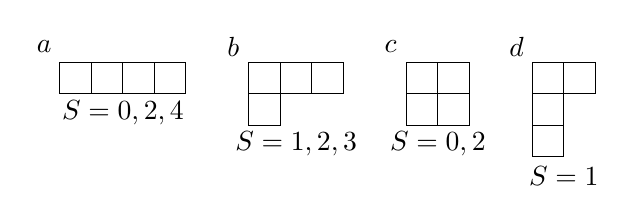
\begin{tikzpicture}[x=4mm,y=4mm,line width=.35pt]
\node at (-.5,.5){$a$};\draw (0,0) rectangle (4,-1);\foreach \x in {1,2,3}\draw (\x,0)--(\x,-1);\node at (2,-1.6){$S=0,2,4$};
\node at (5.5,.5){$b$};\draw (6,0) rectangle (9,-1);\draw (7,0)--(7,-1);\draw (8,0)--(8,-1);\draw (6,-1) rectangle (7,-2);\node at (7.5,-2.6){$S=1,2,3$};
\node at (10.5,.5){$c$};\draw (11,0) rectangle (13,-2);\draw (12,0)--(12,-2);\draw (11,-1)--(13,-1);\node at (12,-2.6){$S=0,2$};
\node at (14.5,.5){$d$};\draw (15,0) rectangle (17,-1);\draw (16,0)--(16,-1);\draw (15,-1) rectangle (16,-3);\draw (15,-2)--(16,-2);\node at (16,-3.6){$S=1$};
\end{tikzpicture}
\end{center}
